% Chapter 4

\chapter{Experiment} % Write in your own chapter title
\label{Chapter4}
\lhead{Chapter 4. \emph{Experiment}}

We set up experiment environment on a desktop which has hardware i7 CPU, 8G RAM and a GeForce GTX 770 and software operation system Ubuntu Linux 14.04. We train models in Caffe\citep{jia2014caffe} which is a open source framework and develop spatial pyramid pooling layer in the architecture.

\section{Training Neural Network}

We trained model with the 1000-category ImageNet2012 on deep learning framework CaffeNet~\cite{jia2014caffe} on a  We use the base network architecture of fast(smaller) model~\cite{ZeilerF13} which achieved an excellent result in 2013 ImageNet Competition. We implement SPP with CUDA C language and deploy them before the first fully-connected layer.

In experiment, a subset of ImageNet dataset, which contains 1.2 million labelled high-resolution images depicting 1000 object categories for training and 50,000 validation images, is used as training dataset. ImageNet contains of multi-scale and some grey images which are converted to a constant input dimensionality. Then images are resized to $256x256$. And for grey images, they are combined it triple to minic a RGB image. Model is trained on the raw RGB values of pixels. Activation function is chosen  Rectified Linear Units(ReLUs), which allows for faster and effective training of deep neural networks.

\begin{equation}\label{eq:ReLU}
f(x) = max(0, x)
\end{equation}

The network model \ref{eq:NetPara} is trained with stochastic gradient descent as backpropagation learning rule, with a batch size of 128, and momentum of 0.9. The weights are initialized from a $0$ mean Gaussian distribution with standard deviation 0.01 in each layer. The neuron biases, in the $Conv_{2}$, $Conv_{4}$, $Conv_{5}$ and fully connected layers, are initialized with the constant 1, while biases in other layers are initialized with constant 0.

The learning rates are set equally for all layers. It was initialized at 0.01 and decreases with stepdown policy which means that it would drop by a factor of 10 after 100000 iteration. In total, the learning rate drops 3 times and accuracy stops after 370K iterations. 

The training was regularised by dropout and weight decay. Dropout regularisation is implemented in the first two fully-connected layers and dropout ratio is set to 0.5. The neurons which are dropped out output zero and do not participate in backpropagation. Therefore, the neural network samples a different architecture each time. It greatly decreases complex co-adaptations of neurons because a neuron cannot depend on the existence of distinct other neurons. For weight decay $\epsilon$, it is set to 0.0005 which means , after each weight update, the new weight is shrunk according to 
\begin{equation}\label{eq:ffEq}
w^{new} = w^{old}(1 - \epsilon)
\end{equation}

\section{Fine-tuning Model}

As mentioned previously, the CNN network is pre-trained with aim of classifying objects in images. However, the target task is to classify weather scene and the pre-trained model contains more than 60 million parameters which are too high for training target model from scratch up, because the target dataset has only 10000 images in total. With the excellent accuracy achieved from previous works about transfer learning, it is a good approach to fine-tune previous model. The previous model does a job to classify 1000 categories and the target model does for two class classification. 

Fine-tuning transfers weights of each layers in previous model to new one except the last fully connected layer. The last layer is taken over by a new one which contains the same amount of neurons as class number in the dataset, say two, and is initialized with random weights. One advantage of fine-tune is that it highly reduces the probability of overfitting  while training with small dataset. The other advantage is the existing weights are close to optimal values and the gradient descent algorithm can converge quickly.

In the problem, we want to classify sunny and cloudy images, then the last layer of the previous architecture, $fc8$, is taken place by a layer with two neurons, one for sunny and one for cloudy. The model, trained using ILSVRC2012 dataset, is used to initialize most weights in the neural network for the fine-tuning experiment. At the same time, $1000$ images are used to evaluate model. The model is fine-tuned in $10000$ iterations which means that total training images are fed into CNN $\frac{128x10000}{9000}=142$ times. The initial base learning rate is 0.001 and the rate is divided by 10 every 10 epochs. Because the weights in $fc8$ are randomly initialized which means they are not close to final optimization value, the learning rate of $fc8$ is 10 times of the base learning rate in order to converge faster.

To minimise risk of overfitting, data augmentation is introduced in to experiment. Different version of patches are generated from each image via simple transformations, for example flipping and cropping. Some practical methods have been implemented and increase accuracy \citep{krizhevsky2012imagenet}. We do this job by increasing the spatial generalization capability of the model  by cropping 5 different patches from four corners and center of images, and flipping them. Totally, we generate 10 different images with the same label.

\section{Companion Experimental}

To compare the performance of fine-tuned model, we do some a experiment with other method. We use a pre-trained model with AlexNet architecture and extract features from fc7. Then we apply SVM on the features and learn a classifier to do weather classification.

\section{Experimental Result}

The results in table\ref{ExpRes} shows that supervised pre-training model have excellent generalization capability. 

\begin{table}[h]
\begin{center}
    \begin{tabular}{| c | c | c | c | c |}
    \hline
    Methods & CNN+SVM & SPP+SVM & Finetune on CNN & Finetune on SPP  \\ \hline
    Accuracy & $84.8\%$ & $82.1\%$ & $93.1\%$ & $93.98\%$ \\ \hline
    \end{tabular}
    \caption{CNN means with original trained model, SPP means model deployed with spatial pyramid pooling layer}
    \label{ExpRes}
\end{center}
\end{table}

The fine-tuning process is very quick, and accuracy rate convergences to over $90\%$. 
After 12 epoch, the accuracy rate exceeds $90\%$. 
\graphicspath{ {./Figures/} }
\begin{figure}[!htb]
    \centering
	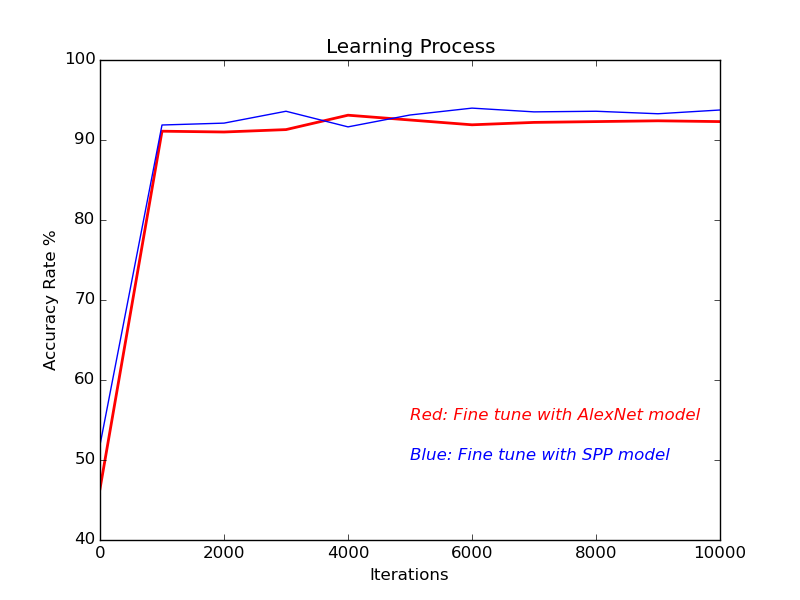
\includegraphics[width=0.8\textwidth]{FinetuneAccuracy.png}
    \caption{Finetune Process}%
    \label{fig:finetuneprocess}%
\end{figure}

No single image dataset can totally capture variation in natural images, so even ImageNet is biased in some fields. Then pre-training may be make the CNN to overfit and then damage model generalization capability. To learning the process of ImageNet pre-training, we look into the effect of pre-training period on generalization performance with and without fine-tuning. In figure \ref{fig:finetuneprocess}, we can find that longer pre-training improves performance.

To have a more detailed information of fine-tuning process, we can have a closer look at training loss. We plot the curve of first 200 iterations and loss value.

\begin{figure}[!htb]
    \centering
	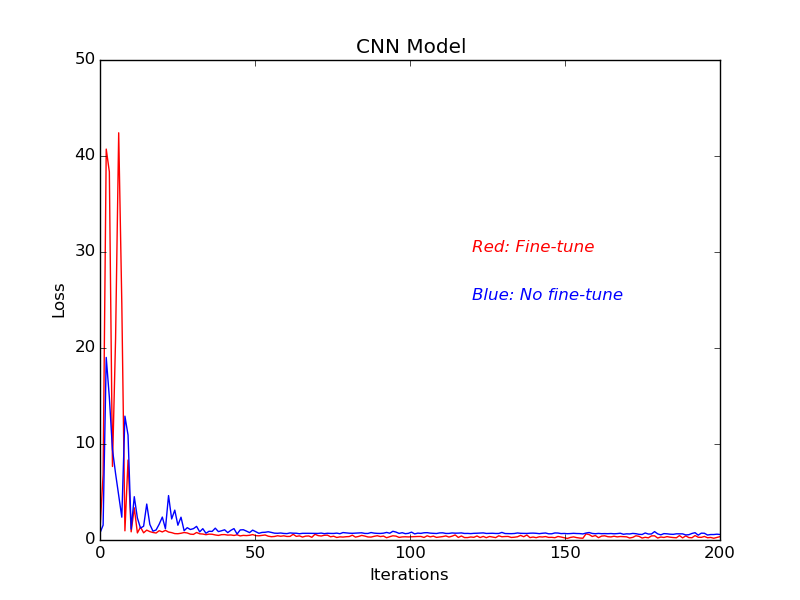
\includegraphics[width=0.4\textwidth]{finetuneCNNProcess.png}
	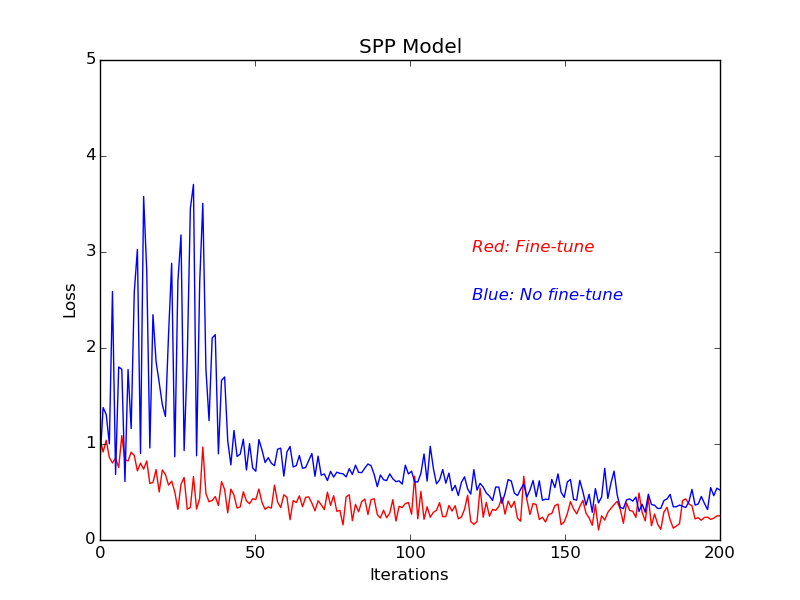
\includegraphics[width=0.4\textwidth]{finetuneSPPProcess.png}
    \caption{Finetune Process}%
    \label{fig:FTvsSC}%
\end{figure}

From figure \ref{fig:FTvsSC}, we can find that the fine-tuning procedure produces a more smooth loss function curve and ceases with a better loss. In the left figure, the loss value of fine tune procedure is higher than no fine tune process at the beginning, then it shrinks sharply and keeps lower. In the other figure, we can find that starting loss value are both less than in the left figure. And the loss values of fine tune are less than no fine tune process. We can conclude that generally fine tune is a effective approach to reduce loss value and fine tune on SPP model can achieve a better result than CNN model.

\begin{figure}[!htb]
    \centering
	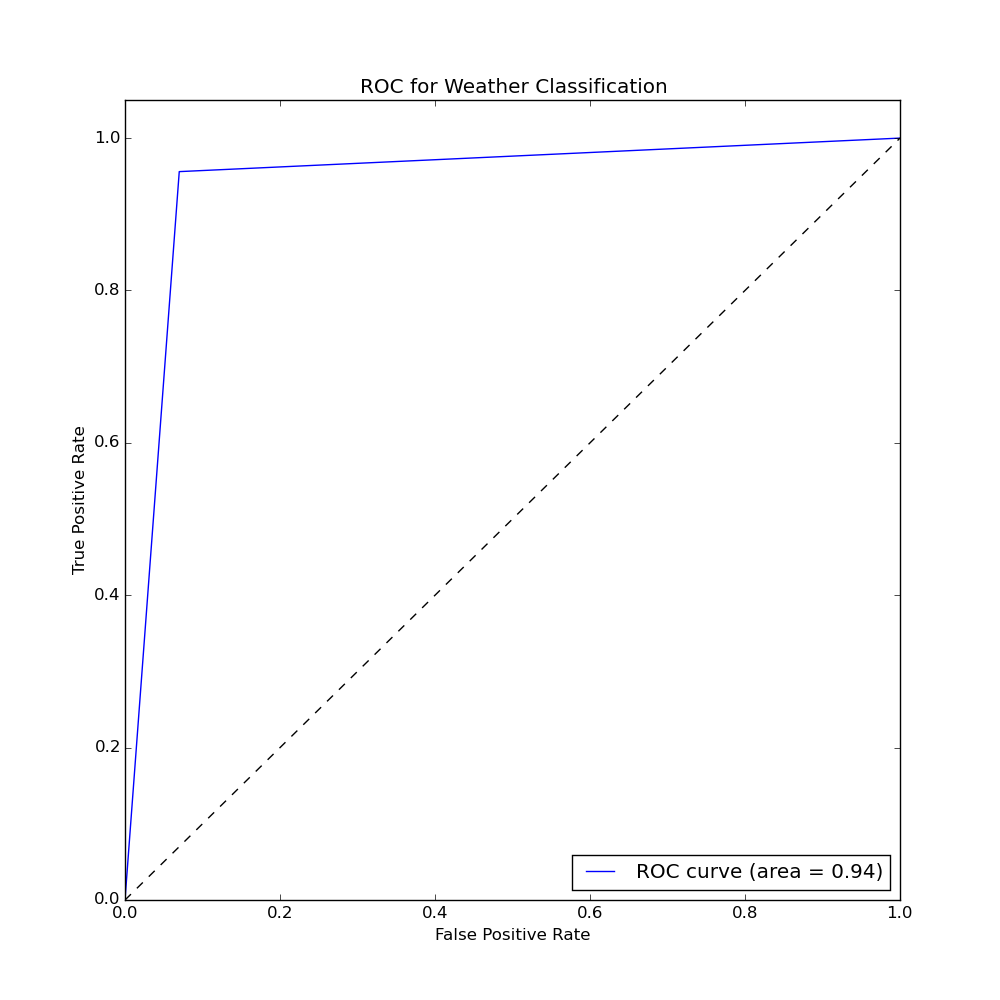
\includegraphics[width=0.8\textwidth]{ROCWeatherClassification.png}
    \caption{ROC Curve}%
    \label{fig:WeatherClassificationROC}%
\end{figure}



\section{Architecture Analysis}

Although CNNs have excellent performance in computer vision field, there is still a long way to understand insight working mechanism. In order to have more insight about the reason why deep layers can increase performance of visual sentiment classification, we will do some analysis on fine-tuned network.

The outputs of each layers have been treated as visual descriptors \citep{razavian2014cnn}, while the vectors are composed by outputs of neurons in previous layer. While the lower layers encode low-level features, top layers have been used to capture high-level information. In other words, we can train classifiers basing on features extracted from each layer.

In fully-connected layer, units can be represented as d dimensional vectors, and no further manipulation is needed. The layer takes all outputs of previous layer ,for example CONV, POOL, NORM,whose feature maps are multidimensional, and flats the feature maps into d dimensional vectors. The outputs of fully connected layer are feed into a classifier. Two types of linear classifiers are used. They are linear Support Vector Machine and Softmax.

We have a look for the feature maps of each convolutional layers a cloudy image.

\graphicspath{ {./Figures/DifferentLayers/} }

\begin{figure}[htb]
    \centering
    \subfigure[raw image]{
		\begin{minipage}{0.3\textwidth}
		   		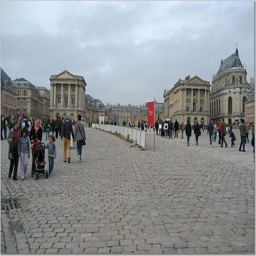
\includegraphics[width=1\textwidth]{cloudy1}
		   		\label{fig:cloudy}
		\end{minipage}
    	} 
    \subfigure[conv1 output]{
		\begin{minipage}{0.3\textwidth}
		   		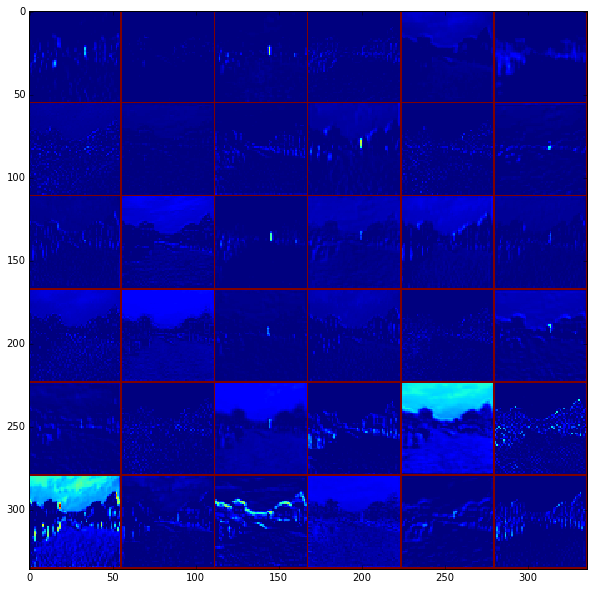
\includegraphics[width=1\textwidth]{cloudy1_conv1_fm}
		   		\label{fig:cloudy_conv1}
		\end{minipage}
    	} 
    \subfigure[conv2 output]{
		\begin{minipage}{0.3\textwidth}
		   		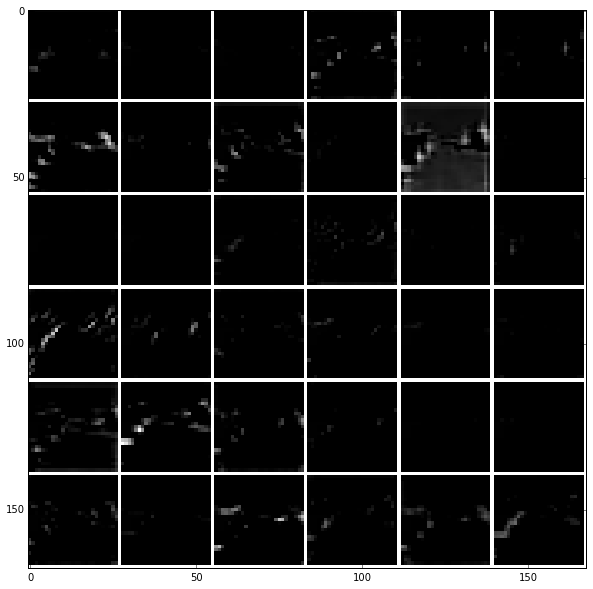
\includegraphics[width=1\textwidth]{cloudy1_conv2_fm}
		   		\label{fig:cloudy_conv2}
		\end{minipage}
    	} 
    \subfigure[conv3 output]{
		\begin{minipage}{0.3\textwidth}
		   		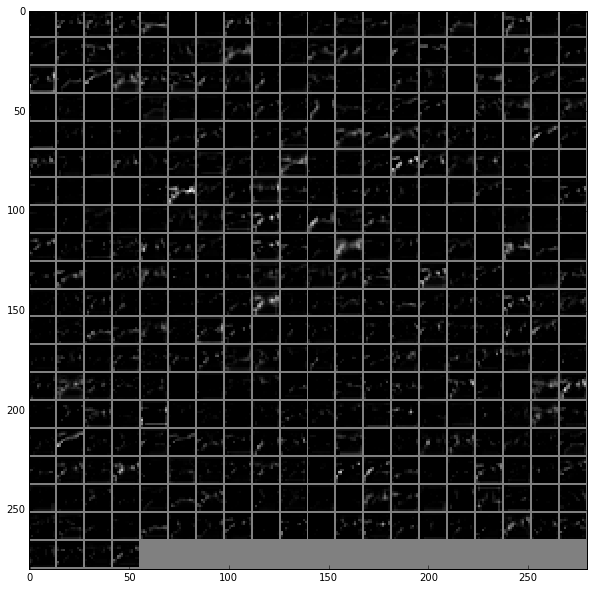
\includegraphics[width=1\textwidth]{cloudy1_conv3_fm}
		   		\label{fig:cloudy_conv3}
		\end{minipage}
    	} 
    \subfigure[conv4 output]{
		\begin{minipage}{0.3\textwidth}
		   		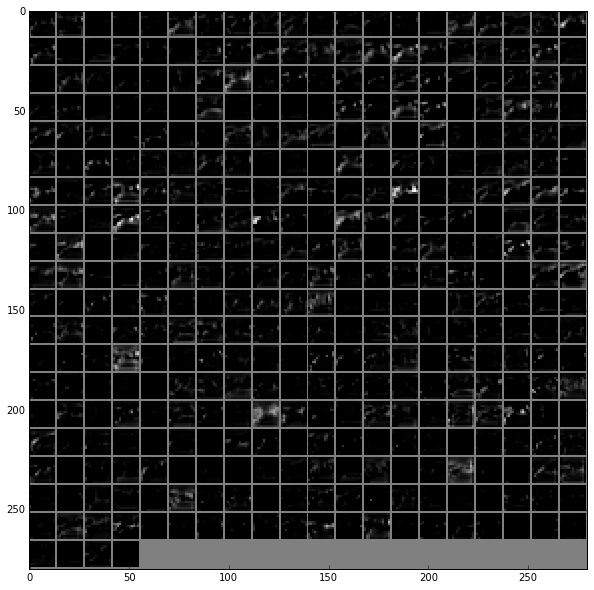
\includegraphics[width=1\textwidth]{cloudy1_conv4_fm}
		   		\label{fig:cloudy_conv4}
		\end{minipage}
    	} 
    \subfigure[conv5 output]{
		\begin{minipage}{0.3\textwidth}
		   		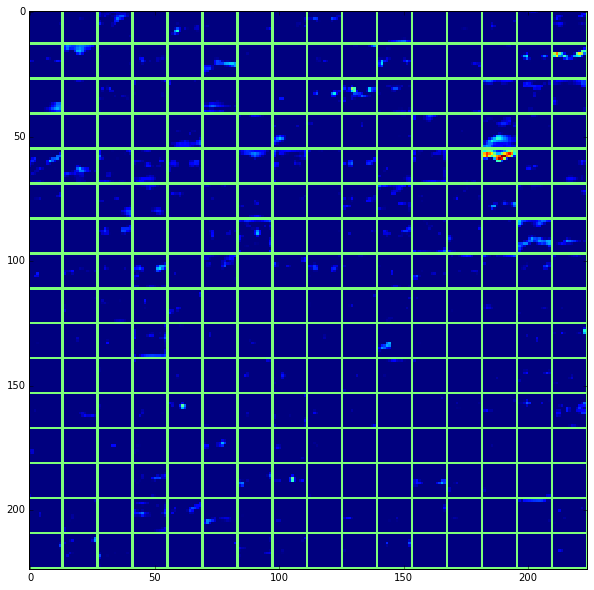
\includegraphics[width=1\textwidth]{cloudy1_conv5_fm}
		   		\label{fig:cloudy_conv5}
		\end{minipage}
    	} 

    \caption{A cloudy image and outputs of convolutional layers}%

    \label{fig:cloudy_finetuneprocess}%
\end{figure}

In Figure \ref{fig:cloudy_finetuneprocess}, a cloudy image is fed into CNN and b-d are outputs of different convolutional layers. For the sake of image size, there are only parts of filters are plotted in images b-d.

Compared to the previous cloudy image, we can have a look for similar outputs of a sunny image.

\begin{figure}[!htb]
    \centering
    \subfigure[raw image]{
		\begin{minipage}{0.3\textwidth}
		   		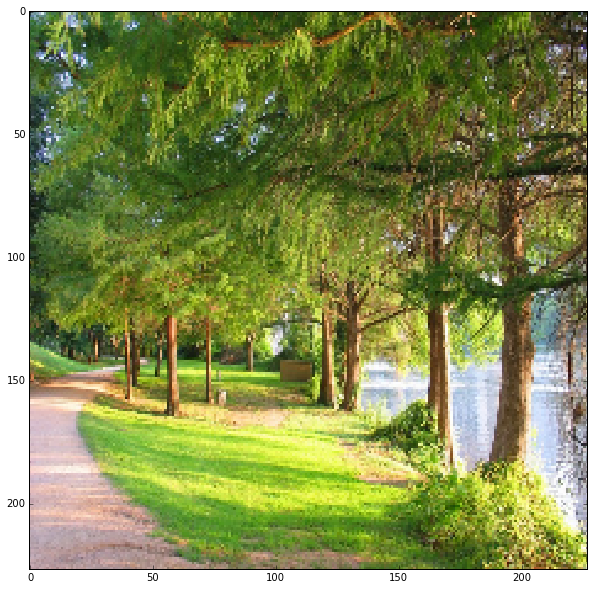
\includegraphics[width=1\textwidth]{sunny2}
		   		\label{fig:sunny}
		\end{minipage}
    	} 
    \subfigure[conv1 output]{
		\begin{minipage}{0.3\textwidth}
		   		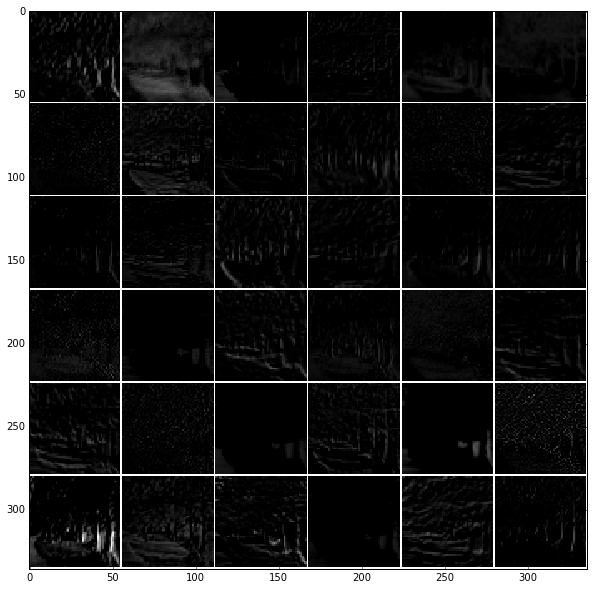
\includegraphics[width=1\textwidth]{sunny2_conv1_fm}
		   		\label{fig:sunny_conv1}
		\end{minipage}
    	} 
    \subfigure[conv2 output]{
		\begin{minipage}{0.3\textwidth}
		   		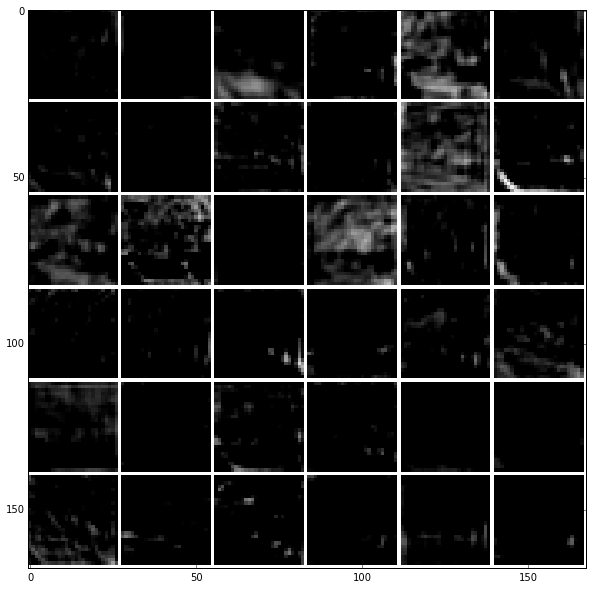
\includegraphics[width=1\textwidth]{sunny2_conv2_fm}
		   		\label{fig:sunny_conv2}
		\end{minipage}
    	} 
    \subfigure[conv3 output]{
		\begin{minipage}{0.3\textwidth}
		   		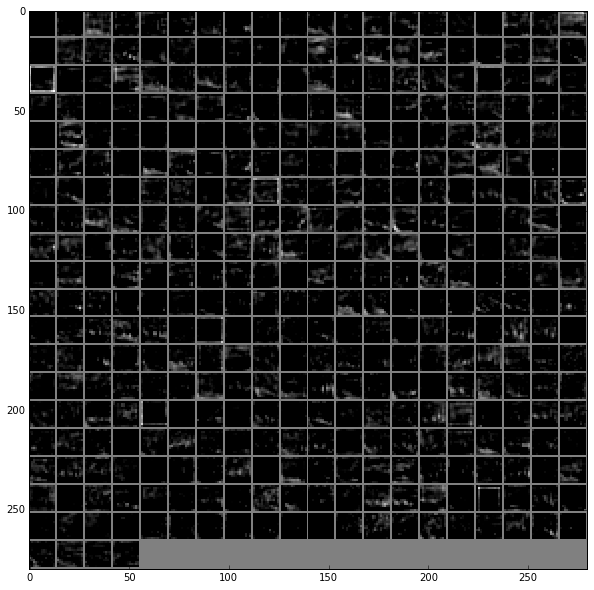
\includegraphics[width=1\textwidth]{sunny2_conv3_fm}
		   		\label{fig:sunny_conv3}
		\end{minipage}
    	} 
    \subfigure[conv4 output]{
		\begin{minipage}{0.3\textwidth}
		   		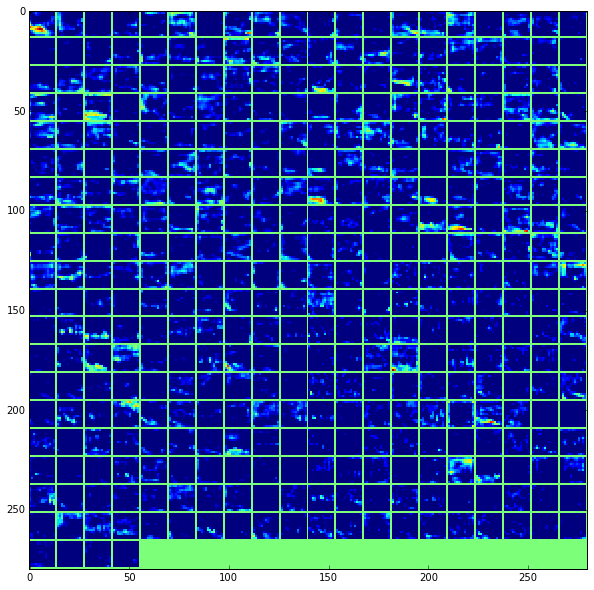
\includegraphics[width=1\textwidth]{sunny2_conv4_fm}
		   		\label{fig:sunny_conv4}
		\end{minipage}
    	} 
    \subfigure[conv5 output]{
		\begin{minipage}{0.3\textwidth}
		   		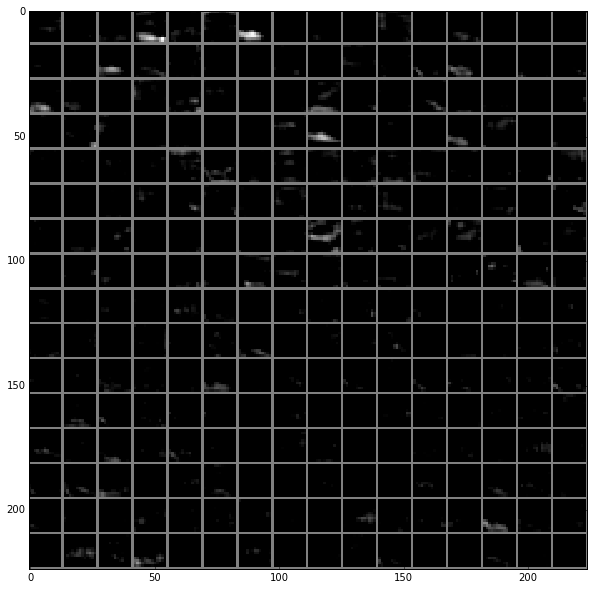
\includegraphics[width=1\textwidth]{sunny2_conv5_fm}
		   		\label{fig:sunny_conv5}
		\end{minipage}
    	} 

    \caption{A sunny image and outputs of convolutional layers}%

    \label{fig:sunny_finetuneprocess}%
\end{figure}

The convolutional layers output the same number filters as Figure \ref{fig:cloudy_finetuneprocess}. Neural activations in fully connected layers can act as d-dimensional vectors, where d is the number of neurons. Not like the earlier layers, for instance CONV and POOLING whose feature maps are multimensional. In figure \ref{fig:ImageNetArch}, we can get that the feature maps of CONV1 are $96\times55\times55$ dimension and the feature maps of CONV5 are $256\times13\times13$ dimension. The feature maps of CONV5 are downsampled by POOL5 and flatten into d-dimensional vectors and used as features for classifier. We can use two types of classifiers. One is linear support vector machine and the other is SoftMax.

\section{Transfer Learning}

Because we do not have sufficient size of dataset, comparing to ImangNet, we use a pretrained model based on ImageNet dataset and then use the CNN either as a fixed feature extractor or an initialization for our task. After fine tuning, weights have been updated for fitting new functions. Accordingly, the feature maps have some difference.

\begin{figure*}[!htb]
\begin{center}

\begin{tabular}{|c|c|c|c|c|c|} \hline\hline
Image & Conv1 & Conv2 & Conv3 & Conv4 & Conv5  \\ \hline
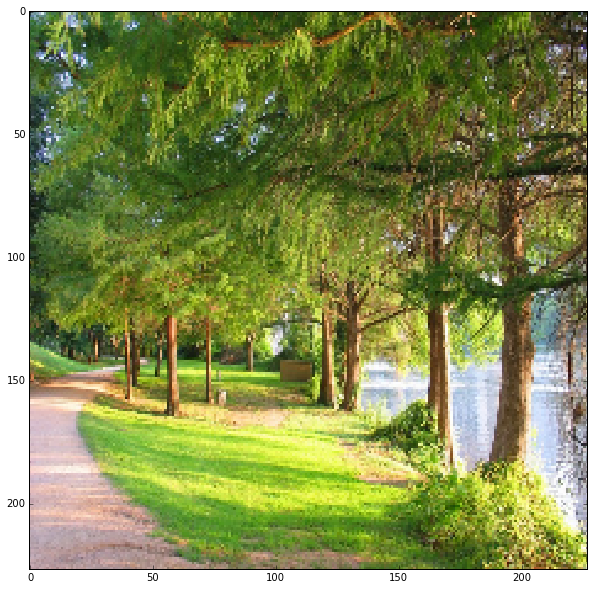
\includegraphics[scale=0.1]{sunny2.png} &
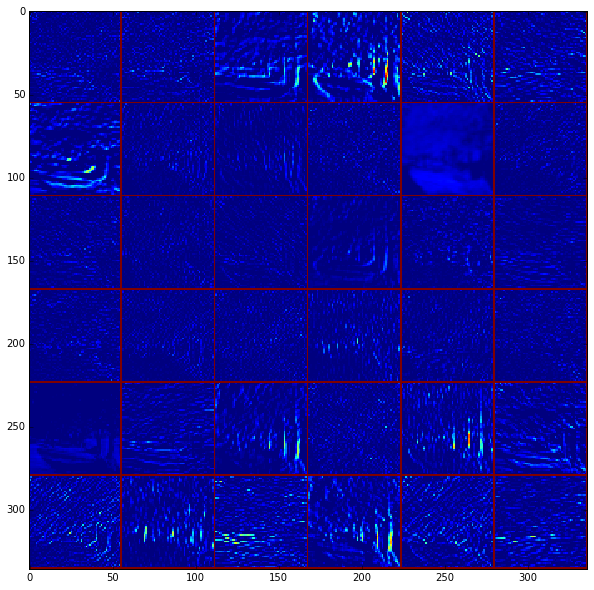
\includegraphics[scale=0.1]{sunny2_caffe_conv1_fm.png} &
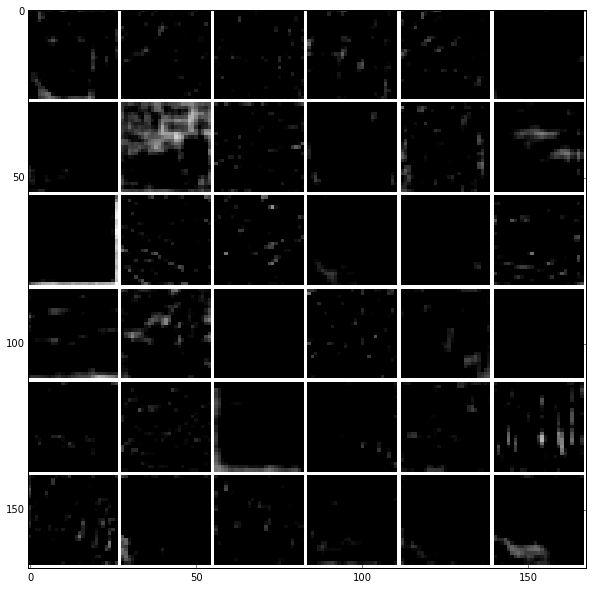
\includegraphics[scale=0.1]{sunny2_caffe_conv2_fm.png} &
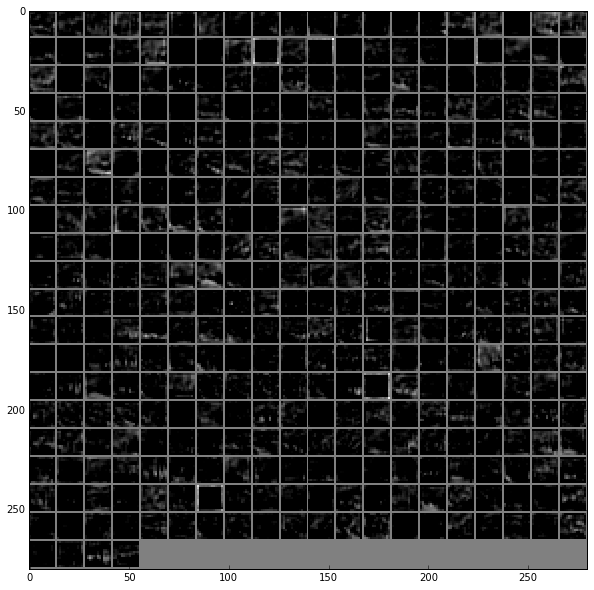
\includegraphics[scale=0.1]{sunny2_caffe_conv3_fm.png} &
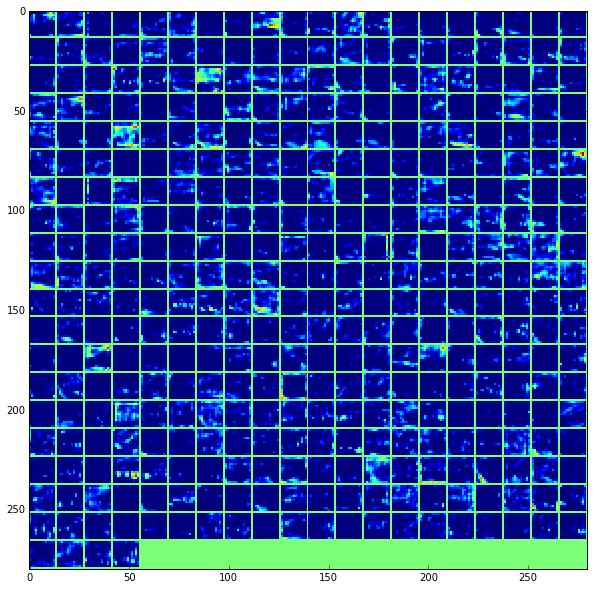
\includegraphics[scale=0.1]{sunny2_caffe_conv4_fm.png} &
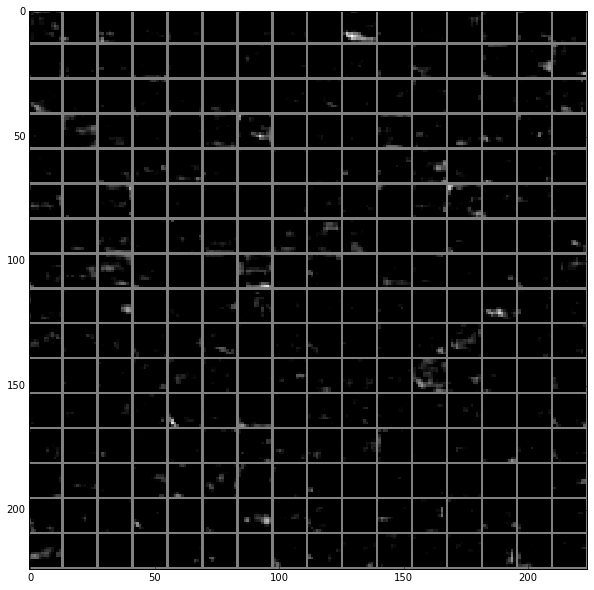
\includegraphics[scale=0.1]{sunny2_caffe_conv5_fm.png}\\ \hline\hline

Image & Conv1 & Conv2 & Conv3 & Conv4 & Conv5  \\ \hline
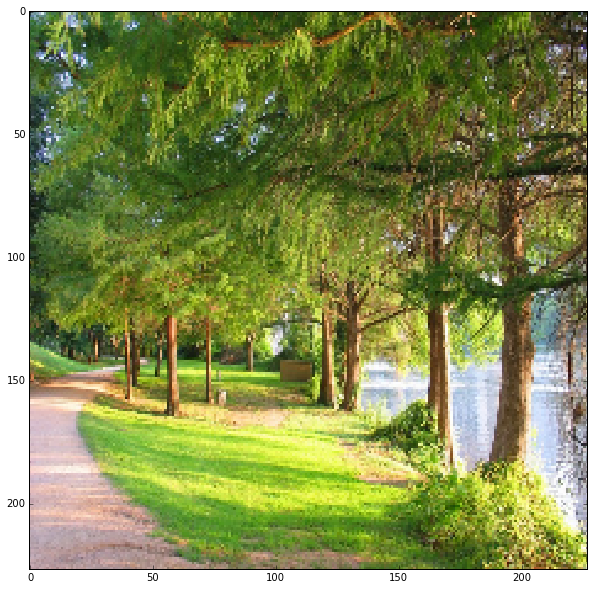
\includegraphics[scale=0.1]{sunny2.png} &
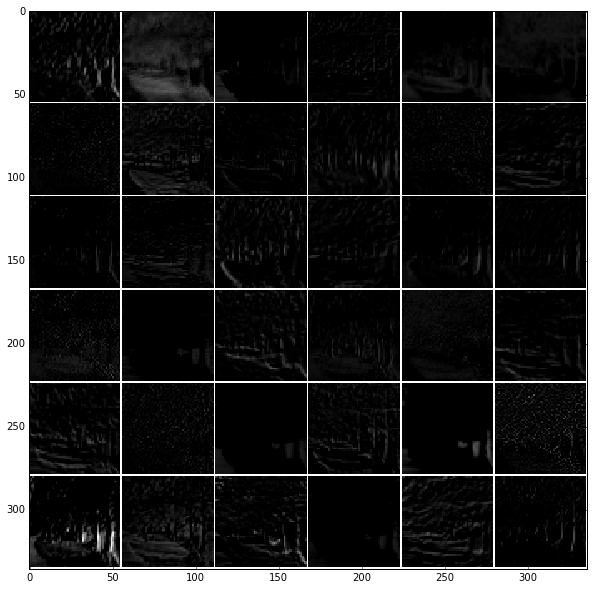
\includegraphics[scale=0.1]{sunny2_conv1_fm.png} &
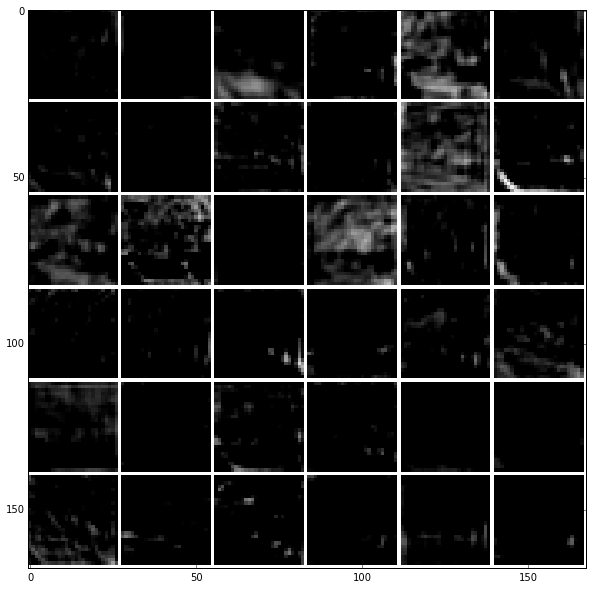
\includegraphics[scale=0.1]{sunny2_conv2_fm.png} &
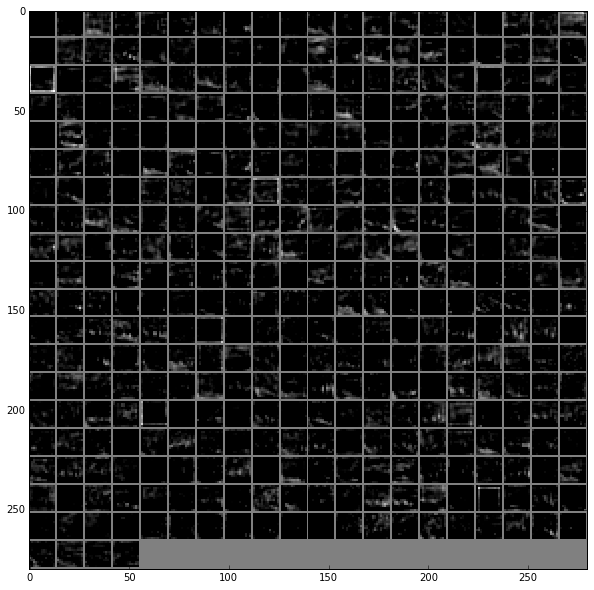
\includegraphics[scale=0.1]{sunny2_conv3_fm.png} &
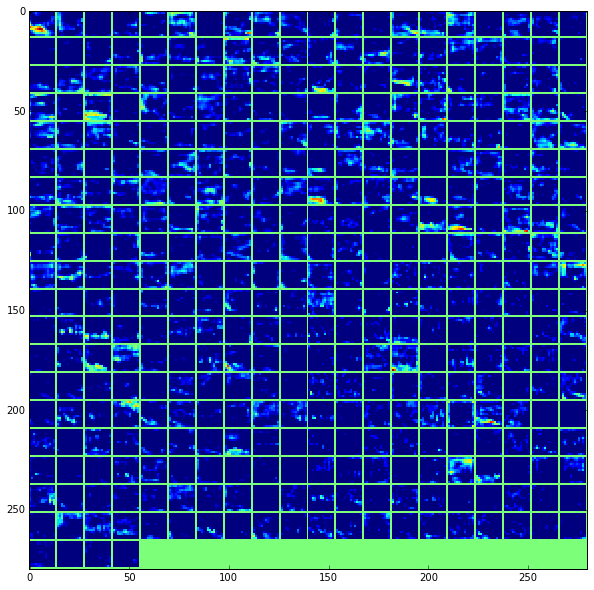
\includegraphics[scale=0.1]{sunny2_conv4_fm.png} &
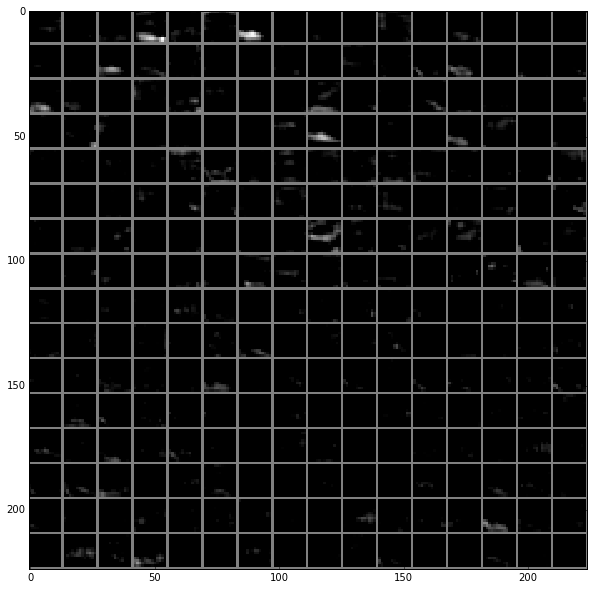
\includegraphics[scale=0.1]{sunny2_conv5_fm.png}\\ \hline\hline
\end{tabular}

\end{center}
	\caption{Visiualization of feature maps outputs between original CNN model and CNN-SPP model. The upper images are from original model and the lower images are from fine tuned model}
	\label{fig:diff_featuremap}%
\end{figure*}

\begin{figure}[htb]
    \centering
	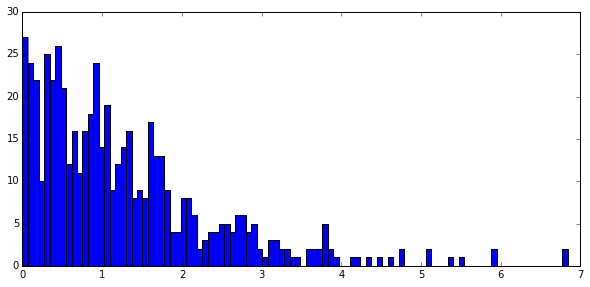
\includegraphics[width=0.4\textwidth]{sunny2_hist_caffe_fc7.png}
	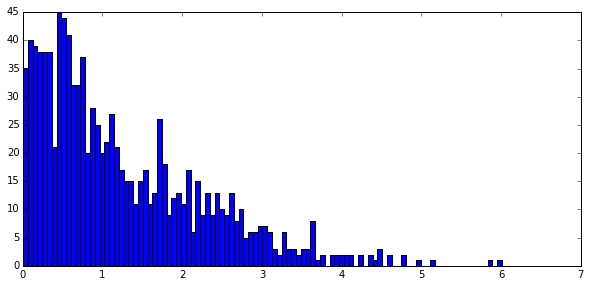
\includegraphics[width=0.4\textwidth]{sunny2_hist_spp_fc7.png}
    \caption{Histogram distribution of vectors from FC7. Left one is from CNN model and right one is from finetuned model}%
    \label{fig:fc7_hist_output}%
\end{figure}

From the feature maps and histogram distribution maps, We can find that the outputs are slightly different. The fine tuned model generates smoother histogram distribution. 

\section{Error Results}

The images \ref{fig:Misclassification} are misclassified. They are hard to judge sunny or cloudy, even for human being.
\graphicspath{ {./Figures/} }
\begin{figure}[htb]
    \centering
    \subfigure[sunny]{
		\begin{minipage}{0.3\textwidth}
		   		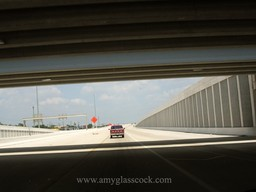
\includegraphics[width=1\textwidth]{err_sunny1}
		   		\label{fig:sunny}
		\end{minipage}
    	} 
    \subfigure[sunny]{
		\begin{minipage}{0.3\textwidth}
		   		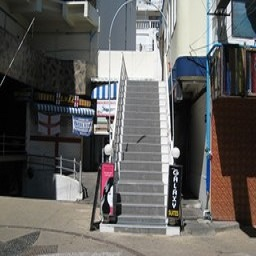
\includegraphics[width=1\textwidth]{err_sunny2}
		   		\label{fig:sunny_conv1}
		\end{minipage}
    	} 
    \subfigure[sunny]{
		\begin{minipage}{0.3\textwidth}
		   		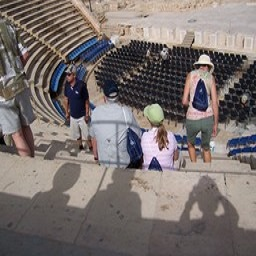
\includegraphics[width=1\textwidth]{err_sunny3}
		   		\label{fig:sunny_conv2}
		\end{minipage}
    	} 
    \subfigure[cloudy]{
		\begin{minipage}{0.3\textwidth}
		   		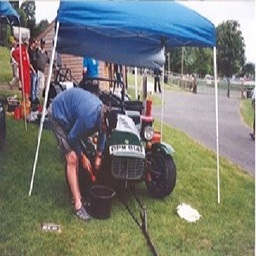
\includegraphics[width=1\textwidth]{err_cloudy1}
		   		\label{fig:sunny_conv3}
		\end{minipage}
    	} 
    \subfigure[cloudy]{
		\begin{minipage}{0.3\textwidth}
		   		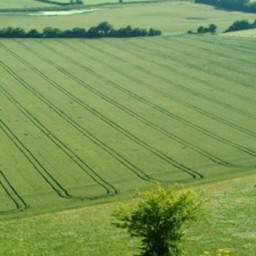
\includegraphics[width=1\textwidth]{err_cloudy2}
		   		\label{fig:sunny_conv4}
		\end{minipage}
    	} 
    \subfigure[cloudy]{
		\begin{minipage}{0.3\textwidth}
		   		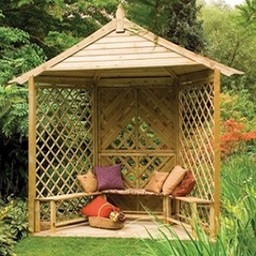
\includegraphics[width=1\textwidth]{err_cloudy3}
		   		\label{fig:sunny_conv5}
		\end{minipage}
    	} 
    \caption{Misclassified images}%
    \label{fig:Misclassification}%
\end{figure}

\section{Conclusion and Future Work}

In this project, we present an approach to do multilabel classification based on neural networks. Although the dataset is manufactured artificially, the experiment shows the strong capacity of neural networks. The project indicates that neural networks are good at approximating difficult function with adjusting topology of network. With the modification on loss function, it is effective to evaluating model which leads the error rates to converge quickly. As future work, we plan to extend approach to the more complicated datasets.